\documentclass{article}
\usepackage{graphicx} % Required for inserting images

\usepackage{darkmode}
\usepackage{tikz}
\enabledarkmode 

\usepackage{geometry}

\usepackage{amsmath}


\geometry{paperwidth=20in, paperheight=20in}

\title{Calc III notes}
\author{Pierson Lipschultz}
\date{March 2025}

\begin{document}

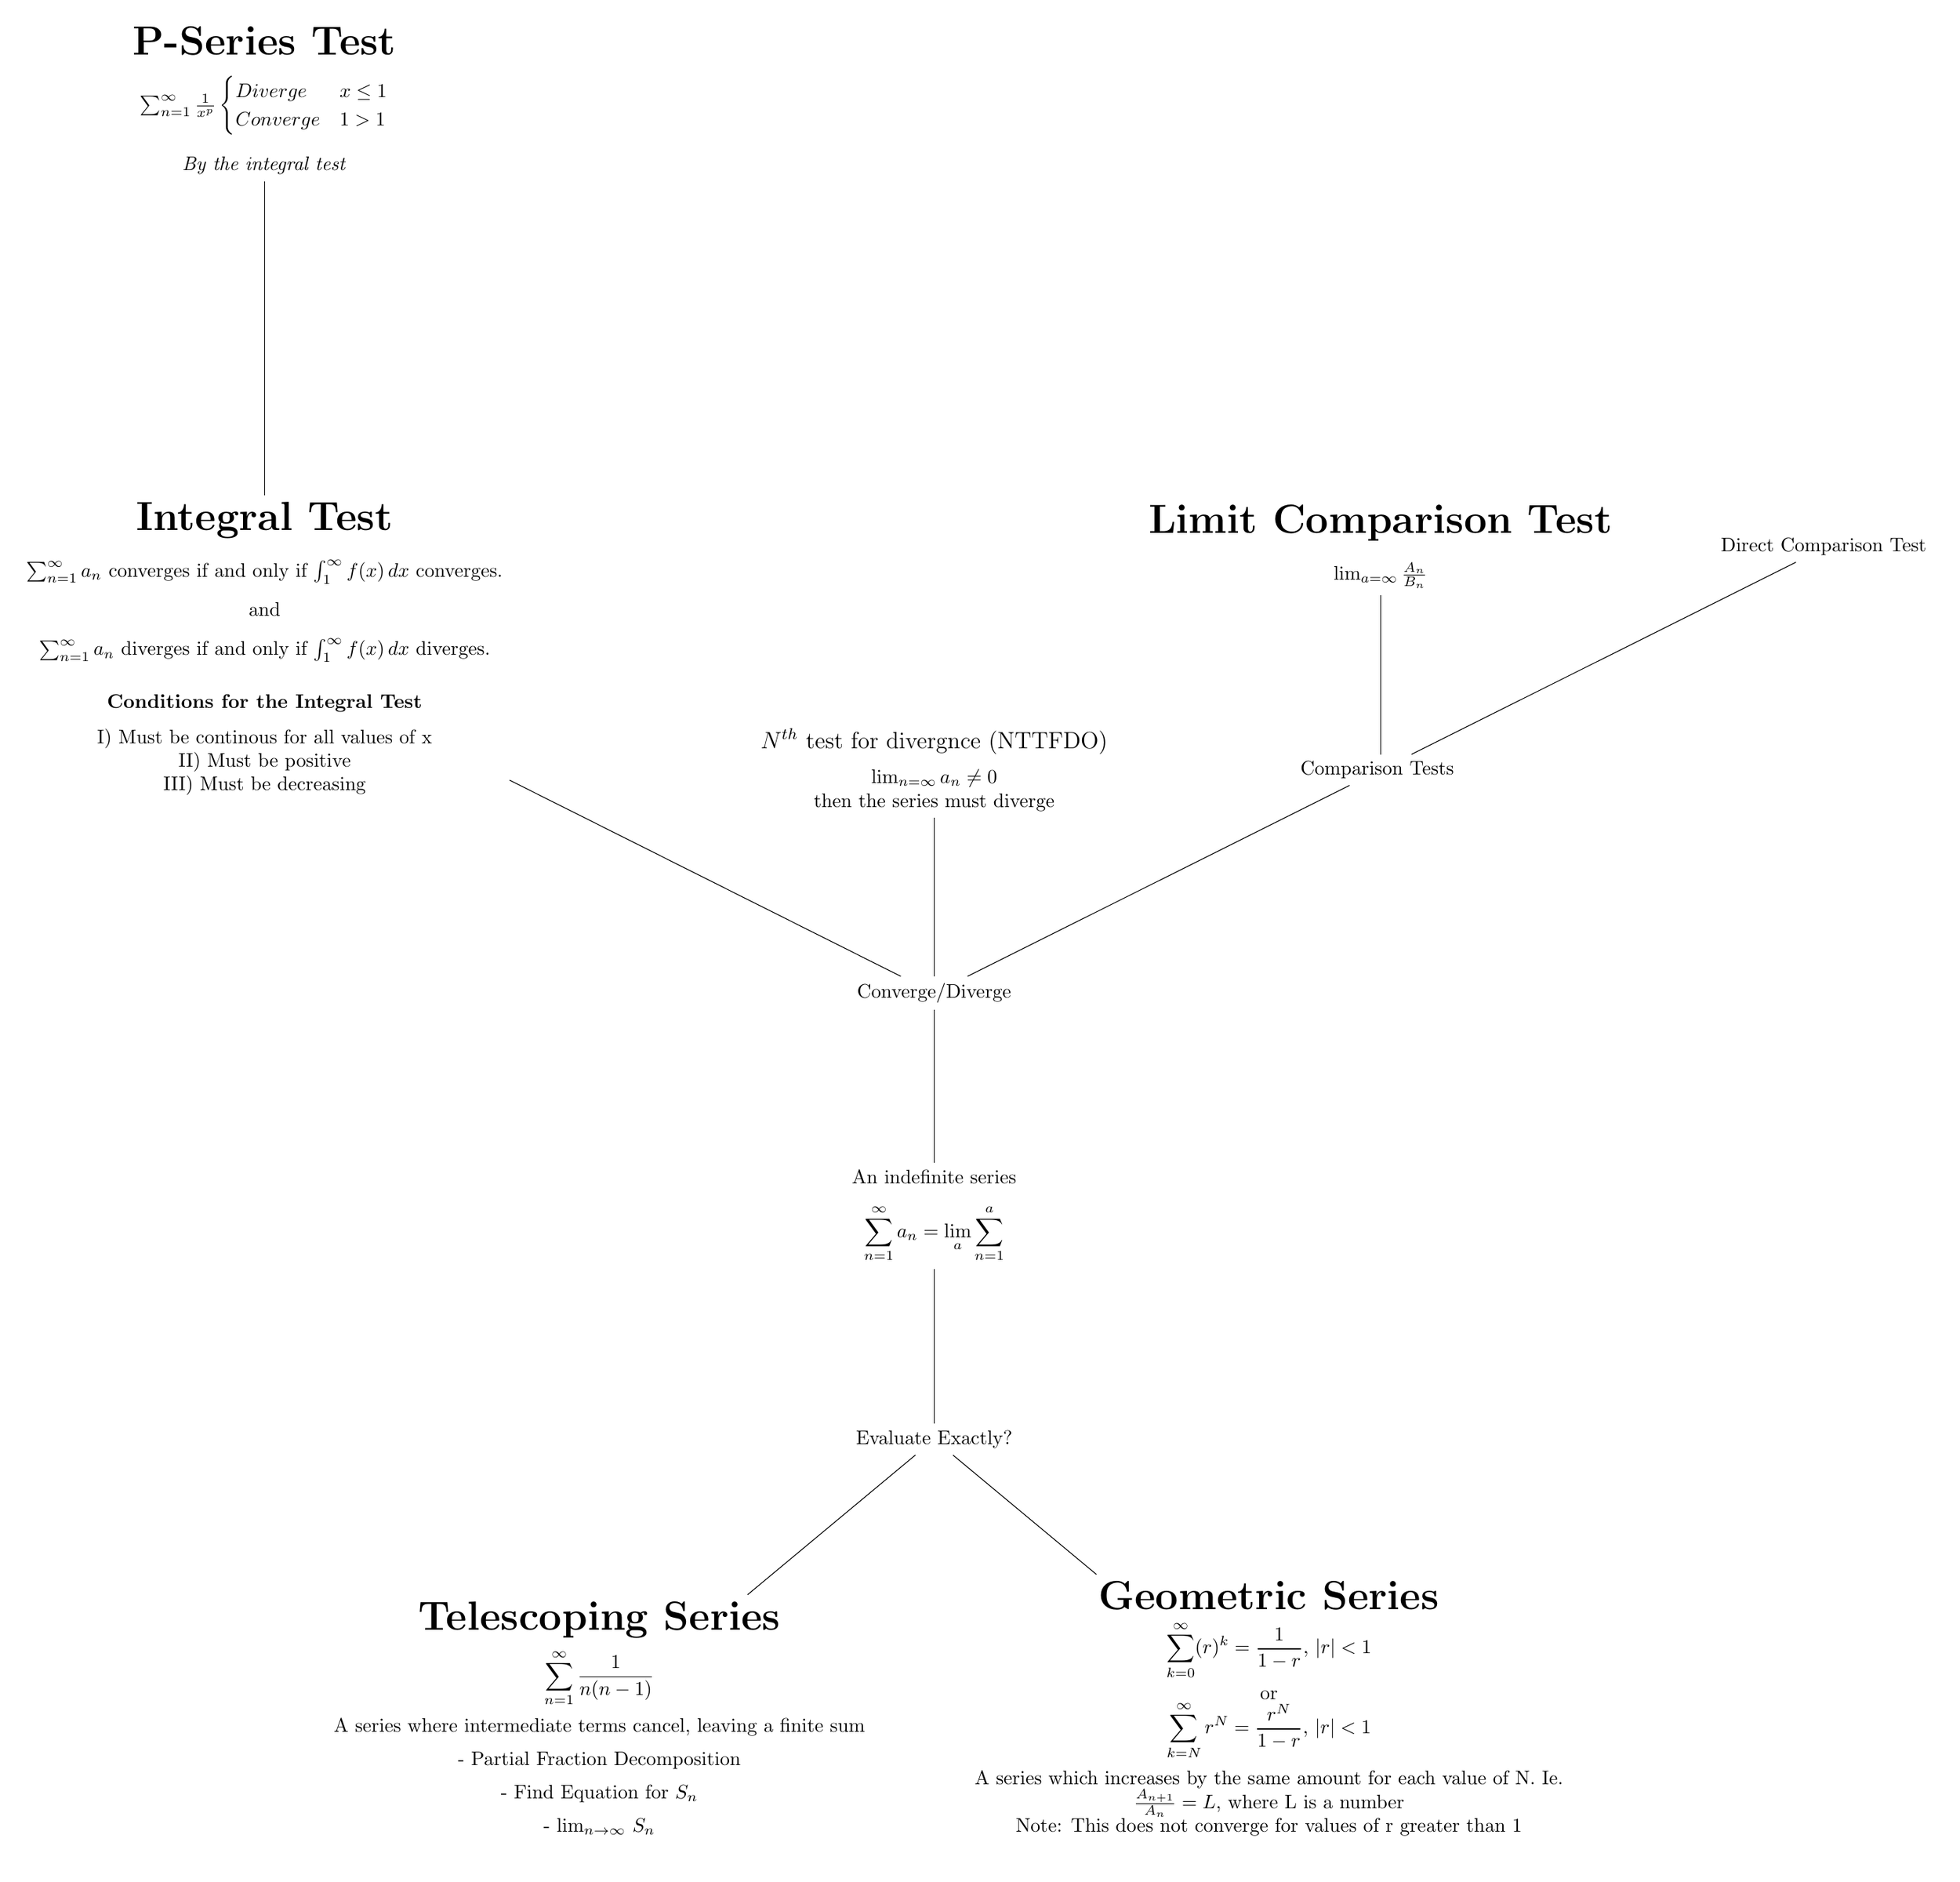
\begin{tikzpicture}

    \node[shape=rectangle, draw=white, align=center] (Main) at (0,0) {
        An indefinite series \\[10pt]
        $\displaystyle \sum_{n=1}^{\infty} a_n = \lim_{a}\sum_{n=1}^{a}$
    };

    \node[shape=rectangle, draw=white] (EvalExc) at (0,-4) {Evaluate Exactly?};


    \node[shape=rectangle, draw=white, align=center] (Tele) at (-6,-9) {
        \textbf{\huge Telescoping Series} \\[5pt]
        $\displaystyle \sum_{n=1}^{\infty} \frac{1}{n(n-1)}$ \\[5pt]
        A series where intermediate terms cancel, leaving a finite sum \\[5pt]
        - Partial Fraction Decomposition  \\[5pt]
        - Find Equation for $S_n$ \\[5pt]
        - $\lim_{n \to \infty}$ $S_n$


    };
    \node[shape=rectangle, draw=white, align=center] (Geom) at (6,-9) {
        \textbf{\huge Geometric Series} \\[5pt]
        $\displaystyle \sum_{k=0}^{\infty} (r)^k = \frac{1}{1-r},$ $|r| < 1 $ \\[5pt] 
        or \\
        $\displaystyle \sum_{k=N}^{\infty} r^N = \frac{r^N}{1-r}, $ $|r| < 1 $\\[5pt]
        A series which increases by the same amount for each value of N. Ie. \\
        $\frac{A_{n+1}}{A_n} = L$, where L is a number \\ 
        Note: This does not converge for values of r greater than 1  \\
    };


    \node[shape = rectangle, draw=white, align=center] (CorD) at (0,4){Converge/Diverge};

    \node[shape = rectangle, draw=white, align=center] (NTTFDO) at (0,8){ \large $N^{th}$ test for divergnce (NTTFDO) \\ [6pt] 
    $\lim_{n=\infty} a_n \neq 0$ \\
    then the series must diverge
    };


    \node[shape = rectangle, draw=white, align=center] (IntTest) at (-12,10){\huge \textbf{Integral Test} \\ [10pt]
    $\sum_{n=1}^{\infty} a_n$ converges if and only if $\int_1^\infty f(x) \, dx$ converges. \\ [8pt]
    and \\ [8pt]
    $\sum_{n=1}^{\infty} a_n$ diverges if and only if $\int_1^\infty f(x) \, dx$ diverges. \\ [15pt]

    \textbf{Conditions for the Integral Test} \\ [6pt]
    I) Must be continous for all values of x\\
    II) Must be positive\\
    III) Must be decreasing \\ 

    };

    \node[shape = rectangle, draw=white, align=center] (PSes) at (-12,20){\huge \textbf{P-Series Test}\\ [10pt]
    
    $\sum_{n=1}^{\infty} \frac{1}{x^p} \begin{cases} 
      Diverge & x\leq 1 \\
      Converge & 1 > 1 \\ 
    \end{cases}$ \\ [10pt]
    
    \textit{By the integral test} 
    };


    \node[shape = rectangle, draw=white, align=center] (CompT) at (8,8){Comparison Tests
    
    };

    \node[shape = rectangle, draw=white, align=center] (LCT) at (8,12){
    {\huge \textbf{Limit Comparison Test}} \\[10pt]
    $\lim_{ a = \infty} \frac{A_n}{B_n} $
    };

    \node[shape = rectangle, draw=white, align=center] (DCT) at (16,12){Direct Comparison Test
    
    };


    \path [-] (Main) edge node[left] {$$} (EvalExc);
    \path [-] (EvalExc) edge node[left] {$$} (Tele);
    \path [-] (EvalExc) edge node[left] {$$} (Geom);
    \path [-] (Main) edge node[left] {$$} (CorD);
    \path [-] (CorD) edge node[left] {$$} (NTTFDO);
    \path [-] (CorD) edge node[left] {$$} (IntTest);
        \path [-] (IntTest) edge node[left] {$$} (PSes);
    \path [-] (CorD) edge node[left] {$$} (CompT);
        \path [-] (CompT) edge node[left] {$$} (LCT);
        \path [-] (CompT) edge node[left] {$$} (DCT);

\end{tikzpicture}

\end{document}
